\documentclass{article}
\usepackage{tikz}

\begin{document}

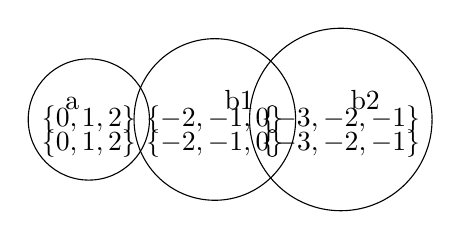
\begin{tikzpicture}[scale=0.8]
    \node[draw,circle] (a) at (0,0) {$\{0,1,2\}$};
    \node[draw,circle] (b1) at (2,0) {$\{-2,-1,0\}$};
    \node[draw,circle] (b2) at (4,0) {$\{-3,-2,-1\}$};

    \node[above left] at (a) {a};
    \node[above right] at (b1) {b1};
    \node[above right] at (b2) {b2};

    \fill[gray!20] (a) -- (b1) -- (b2) -- cycle;
    
    \node[below] at (a) {$\{0,1,2\}$};
    \node[below] at (b1) {$\{-2,-1,0\}$};
    \node[below] at (b2) {$\{-3,-2,-1\}$};
\end{tikzpicture}

\end{document}